\documentclass[10pt,a4paper,twoside]{article}
\usepackage[utf8]{inputenc}
\usepackage[francais]{babel}
\usepackage[T1]{fontenc}
\usepackage{graphicx}
\author{Victor Lezaud}
\title{TD - Modélisation des données}

\begin{document}
\renewcommand{\partname}{Séance de Travaux Dirigés}
\renewcommand{\contentsname}{Sommaire}

\maketitle
\setcounter{tocdepth}{1}
\tableofcontents

\newpage

\part{Langages relationnels}
\section{Bornes des cardinaux}
Soient $R$ un symbole de relation , $r$ et $s$ deux relations $R$, $A \in schema(R)$, $c \in dom(A)$ et $F$ une formule sur $R$. Donner des bornes aux cardinaux des expressions suivantes en fonction de $|r|$ et $|s|$ :

\subsection{Sélection}
$0 \leq |\sigma_{F}(r)| \leq |r|$
\subsection{Union}
$max(|r|,|s|) \leq |r \cup s| \leq |r| + |s|$
\subsection{Soustraction}
$0 \leq |r \setminus s| \leq |r|$
\subsection{Projection}
$1 \leq |\pi_{\{A\}}(r)| \leq |r|$ si $|r| \geq 1$
\subsection{Division}
$0 \leq |r ./ s| \leq |r|/|s|$

\section{Calcul relationnel autorisé}
Soit $Q = \{<x:A, y:B> \mid F(x,y)\}$ une requête du calcul relationnel sur $R$ avec $schema(R) = \{A,B\}$. On considère les formules suivantes :

\subsection{$F(x,y) = R(x,2) \vee R(3,y)$}
\subsubsection{$Q$ est-elle bien formée ?}
$F$ est une combinaison de formule atomique lié par l'opérateur OU, $Q$ est donc bien formée.

\subsubsection{$Q$ est-elle autorisée ?}
Les variables $x$ et $y$ sont des variables libres, or $y$ est négatif dans $R(x,2)$ et $x$ est négatif dans $R(3,y)$, donc par l'opérateur OU $x$ et $y$ sont négatifs donc $Q$ n'est pas autorisé.

\subsubsection{Soit $r_{0}$ une relation sur $R$. $Ans(Q,\{r_{0}\})$ est-il toujours fini ?}
N'importe quel $y \in B$ vérifie la condition $R(x,2)$ si $x \in r_{0}[A]$ et inversement n'importe quel $x \in A$ vérifie la condition $R(3,y)$ si $y \in r_{0}[B]$. Ainsi si $r_{0}$ n'est pas vide $|Ans(Q,\{r_{0}\})| \geq |A|+|B|$, donc $Ans(Q,\{r_{0}\})$ n'est donc pas toujours fini.
\subsubsection{Existe-t-il une requête équivalente en algèbre relationnelle ? en SQL?}
Contrairement au calcul relationnel, l'algèbre relationnelle et le SQL travaille directement sur les relations et ne peuvent donc pas avoir de résultats qui n'appartiennent à aucune relation.

\subsection{$F(x,y) = (R(x,2) \vee R(3,y)) \wedge R(x,y)$}
\subsubsection{$Q$ est-elle bien formée ?}
$F$ est une combinaison de formule atomique lié par les opérateurs OU et ET, $Q$ est donc bien formée.

\subsubsection{$Q$ est-elle autorisée ?}
Les variables $x$ et $y$ sont des variables libres, or $x$ et $y$ sont positifs dans $R(x,y)$, donc par l'opérateur ET $x$ et $y$ sont positifs donc $Q$ est autorisé.

\subsubsection{Soit $r_{0}$ une relation sur $R$. $Ans(Q,\{r_{0}\})$ est-il toujours fini ?}
$Q$ est une formule de calcul autorisée donc $Ans(Q,\{r_{0}\})$ est toujours finie.

\subsubsection{Existe-t-il une requête équivalente en algèbre relationnelle ? en SQL?}
\begin{itemize}
\item Algèbre relationnelle : $\sigma_{B=2\ OU\ A=3}(r_{0})$
\item SQL : \verb[SELECT * FROM r0 WHERE B=2 OR A=3[
\end{itemize}

\subsection{$F(x,y) = \exists x' : A(R(x,y)\wedge R(x',y) \wedge \neg(x=x')) $}
\subsubsection{$Q$ est-elle bien formée ?}
$F$ est une combinaison de formules atomiques liées par les opérateurs NOT et ET, $Q$ est donc bien formée.

\subsubsection{$Q$ est-elle autorisée ?}
Les variables $x$ et $y$ sont des variables libres et $x'$ est déclaré par $\exists x' :A$, or $x$, $y$ et $x'$  sont positifs dans $R(x,y) \wedge R(x',y)$, donc par l'opérateur ET $x$, $x'$ et $y$ sont positifs donc $Q$ est autorisé.

\subsubsection{Soit $r_{0}$ une relation sur $R$. $Ans(Q,\{r_{0}\})$ est-il toujours fini ?}
$Q$ est une formule de calcul autorisée donc $Ans(Q,\{r_{0}\})$ est toujours finie.

\subsubsection{Existe-t-il une requête équivalente en algèbre relationnelle ? en SQL?}
\begin{itemize}
\item Algèbre relationnelle : $\pi_{\{R\}}(\sigma_{A\neq A'}(r_{0} \bowtie \rho_{A\rightarrow A'}(r_{0}))$
\item SQL : \verb[SELECT A,B FROM r0, r0 as r1 WHERE r0.B=r1.B AND r0.A<>r1.B[
\end{itemize}

\subsection{$F(x,y) = \forall z : A(\forall t:B(\neg R(z,t)\vee R(t,z))) $}
\subsubsection{$Q$ est-elle bien formée ?}
$F$ est une combinaison de formules atomiques liées par les opérateurs NOT et OU, $Q$ est donc bien formée.

\subsubsection{$Q$ est-elle autorisée ?}
Les variables $x$ et $y$ sont des variables libres, or $x$ et $y$ n'apparaissent pas dans $F$, $Q$ n'est donc pas autorisée.

\subsubsection{Soit $r_{0}$ une relation sur $R$. $Ans(Q,\{r_{0}\})$ est-il toujours fini ?}
$x$ et $y$ n'apparaissent dans $F$ donc soit $Ans(Q,r_\{{0}\}) = \emptyset$ soit $Ans(Q,\{r_{0}\}) = A \times B$. Ainsi $Ans(Q,\{r_{0}\})$ n'est pas toujours fini.

\subsubsection{Existe-t-il une requête équivalente en algèbre relationnelle ? en SQL?}
NON


\section{Équivalence des langages de requête}
Soient $R$, $S$ deux symboles de relation avec $schema(R) = \{A,B,C,D\}$ et $schema(S)=\{C,E\}$ et soient $r_{1}$, $r_{2}$ deux relations sur $R$ et $s$ une relation sur $S$. Pour chacune des requêtes ci-dessous, donnez les requêtes équivalentes dans les langages vus en cours.

\subsection{$\pi_{\{A,B\}}(r_{1})\cup \pi_{\{A,B\}}(r_{2})$}
\subsubsection{Calcul relationnel}
$Ans(Q,\{r_{1}\}) \cup Ans(Q,\{r_{2}\})$ avec $Q = \{<x:A, y:B> \mid \exists z:C(\exists t:D(R(x,y,z,t))\}$

\subsubsection{SQL}
\begin{verbatim}
SELECT A,B
FROM r1
UNION
SELECT A,B
FROM r2
\end{verbatim}

\subsection{$\pi_{\{A,B\}}(r_{1} \cup r_{2})$}
\subsubsection{Calcul relationnel}
$Ans(Q,\{r_{1} \cup r_{2}\})$ avec $Q = \{<x:A, y:B> \mid \exists z:C(\exists t:D(R(x,y,z,t))\}$

\subsubsection{SQL}
\begin{verbatim}
SELECT A,B
FROM r1 UNION r2
\end{verbatim}

\subsection{$Ans(Q,\{r_{1},s\})$ avec $Q=\{<x:A,y:B> \mid \exists z:C(\exists t:D(R(x,y,z,t) \wedge \exists u:E(S(z,u) \wedge u=t)))\}$}
\subsubsection{Algèbre relationnelle}
$\pi_{\{A,B\}}(r_{1} \bowtie \rho_{E \rightarrow D}(s))$

\subsubsection{SQL}
\begin{verbatim}
SELECT A,B
FROM r1,s
WHERE r1.C = s.C AND D = E
\end{verbatim}


\section{Équivalence de requête}
Soient $R$ et $U$ des symboles de relation avec $schema(R)=\{A,B,C,D\}$ et $schema(U)=\{C,D\}$. On considère une base de données contenant les relations $r$, $s$ et $v$ sur $R$ et $u$ sur $U$.

\subsection{Donner une preuve des équivalences suivantes :}
\subsubsection{$\pi_{\{A,B\}}(r \cup s) = \pi_{\{A,B\}}(r) \cup \pi_{\{A,B\}}(r)$}
\begin{flushleft}
Soit $t$ un tuple sur $\{A,B\}$.\\
$t \in \pi_{\{A,B\}}(r \cup s)$\\
$\Leftrightarrow \exists t'\in r \cup s\ avec\ t'[A,B] = t $\\
$\Leftrightarrow \exists t'\in r\ avec\ t'[A,B] = t\ ou\ \exists t''\in s\ avec\ t''[A,B] = t$
$\Leftrightarrow t \in \pi_{\{A,B\}}(r)\ ou\ t \in \pi_{\{A,B\}}(s)$\\
$\Leftrightarrow t \in \pi_{\{A,B\}}(r) \cup \pi_{\{A,B\}}(s)$
\end{flushleft}

\subsubsection{$ r \cap (s \setminus v)=(r\cap s) \setminus (r\cap v) $}
\begin{flushleft}
Soit $t$ un tuple sur $R$\\
$t \in r \cap (s \setminus v)$\\
$\Leftrightarrow t \in r\ et\ (t \in s\ et\ t \not\in v)$\\
$\Leftrightarrow (t \in r et t \in s)\ et\ (t \not\in v\ et\ t \in r)$\\
$\Leftrightarrow t \in r \cap s\ et\ (t \in r\ et\ t \not\in r\cap t)$\\
$\Leftrightarrow t \in (r\cap s) \setminus (r\cap v)$
\end{flushleft}

\subsubsection{$(r \div u) \cap (s \div u) = (r \cap s) \div u$}
\begin{flushleft}
Soit $t$ un tuple sur $\{A,B\}$\\
$t \in  (r \div u) \cap (s \div u)$\\
$\Leftrightarrow \forall x:ADOM(u), \exists t'\in r\ avec\ t'[A,B]=t\ et\ t'[U] = x\ et\ \forall y:ADOM(u), \exists t''\in s\ avec\ t''[A,B]=t\ et\ t''[U] = y$\\
$\Leftrightarrow \forall x:ADOM(u), \exists t'\in r, t''\in s\ avec\ t'[A,B]=t=t''[A,B]\ et\ t'[U]=x=t''[U] $\\
$\Leftrightarrow  \forall x:ADOM(u), \exists t'\in r \cap s\ avec\ t'[A,B]=t\ et\ t'[U]=x$\\
$\Leftrightarrow t \in (r \cap s) \div u$\
\end{flushleft}

\subsection{Donner un contre-exemple aussi concis que possible pour les équivalences suivantes :}
Pour les prochaines questions nius considèrerons la base de données suivantes:\\

\begin{tabular}{c|cccc}
r & A & B & C & D \\ 
\hline 
 & 0 & 0 & 0 & 0 \\ 
\end{tabular} 
\bigskip
\begin{tabular}{c|cccc}
u & A & B & C & D \\ 
\hline 
 & 0 & 0 & 1 & 1 \\ 
\end{tabular} 
\bigskip
\begin{tabular}{c|cc}
s & C & D \\ 
\hline 
 & 0 & 0 \\
 & 1 & 1 \\ 
\end{tabular} 

\subsubsection{$\pi_{\{A,B\}}(r \setminus s) = \pi_{\{A,B\}}(r) \setminus \pi_{\{A,B\}}(s)$}
\begin{flushleft}
$\pi_{\{A,B\}}(r \setminus s) = \{(0,0)\}$\\
$\pi_{\{A,B\}}(r) \setminus \pi_{\{A,B\}}(s) = \emptyset$\\
\end{flushleft}

\subsubsection{$\pi_{\{A,B\}}(r \cap s) = \pi_{\{A,B\}}(r) \cap \pi_{\{A,B\}}(s)$}
\begin{flushleft}
$\pi_{\{A,B\}}(r \cap s) = \emptyset$\\
$\pi_{\{A,B\}}(r) \cap \pi_{\{A,B\}}(s) = \{(0,0)\}$\\
\end{flushleft}

\subsubsection{$(r \div u) \cup (s \cup u) = (r \cup s) \div u$}
\begin{flushleft}
$(r \div u) \cup (s \cup u) = \emptyset$\\
$(r \cup s) \div u = \{(0,0)\}$\\
\end{flushleft}

\newpage
\part{Algèbre, Calcul relationnel et SQL}
Soit $U=\{num, cnom, pnom, qte, ville, fnom, prix, status\}$ un univers. On définit $R$ un symbole de base de données sur $U$ avec $schema(R)=\{Commande, Fournisseur, Produit\}$ et $schema(Commande)=\{num, cnom, pnom, qte\}$, $schema(Fournisseur)=\{fnom, status, ville\}$, $schema(Produit)=\{pnom, fnom, prix\}$. On considère la base de données $d$ sur $R$ avec $d=\{commandes, fournisseurs, produits\}$ rempli tel que ci dessous:

\begin{tabular}{c|cccc}
commandes & num & cnom & pnom & qte \\ 
\hline 
 & 1535 & Jean & Cornas & 6 \\ 
 & 1854 & Jean & Bordeaux & 20 \\ 
 & 1254 & Paul & Chablis & 20 \\ 
 & 1259 & Paul & Chablis & 25 \\ 
 & 1596 & Paul & Cornas & 12 \\ 
\end{tabular} 

\begin{tabular}{c|ccc}
fournisseurs & fnom & status & ville \\ 
\hline 
 & Vini & SARL & Dijon \\ 
 & BonVin & SA & Dijon \\ 
 & Chapoutier & SA & Valence \\ 
 & SaV & Association & Antraôgues \\ 
\end{tabular} 

\begin{tabular}{c|ccc}
produits & pnom & fnom & prix \\ 
\hline 
 & Cornas & BonVin & 20 \\ 
 & Cornas & Chapoutier & 18 \\ 
 & Bordeaux & Vini & 8.2 \\ 
 & Boudes & Vini & 4.3 \\ 
 & Bordeaux & Chapoutier & 18.5 \\ 
 & Chapoutier & Chapoutier & 5.1 \\ 
 & Chablis & Chapoutier & 5 \\ 
\end{tabular} 

\section{Requête dans les trois langages}
Pour chaque question ci-dessous, donner une expression en algèbre relationnelle, calcul relationnel autorisé et SQL.

\subsection{Donner les informations sur toutes les commandes}
\subsubsection{Algèbre relationnelle}
$commandes$
\subsubsection{Calcul relationnel autorisé}
$ans(Q,\{commandes\})$ avec $Q=\{<x:num,y:cnom,z:pnom,t:qte> \mid Commande(x,y,z,t)\}$
\subsubsection{SQL}
\begin{verbatim}
SELECT * 
FROM commandes
\end{verbatim}

\subsection{Donner le nom de tous les produits commandés}
\subsubsection{Algèbre relationnelle}
$\pi_{\{pnom\}}(commandes)$
\subsubsection{Calcul relationnel autorisé}
$ans(Q,\{commandes\})$ avec $Q=\{<x:pnom> \mid \exists a:num(\exists b:conm(\exists c:qte(Commande(a,b,x,c))))\}$
\subsubsection{SQL}
\begin{verbatim}
SELECT pnom 
FROM commandes
\end{verbatim}

\subsection{Donner le nom des produits commandés par Jean}
\subsubsection{Algèbre relationnelle}
$\pi_{\{pnom\}}(\sigma_{cnom='Jean'}(commandes))$
\subsubsection{Calcul relationnel autorisé}
$ans(Q,\{commandes\})$ avec $Q=\{<x:pnom> \mid \exists a:num(\exists b:qte(Commande(a,'Jean',x,b)))\}$
\subsubsection{SQL}
\begin{verbatim}
SELECT pnom 
FROM commandes
WHERE cnom = 'Jean'
\end{verbatim}

\subsection{Donner le nom des fournisseurs de Bordeaux ou de Cornas à un prix égal à 10 euros}
\subsubsection{Algèbre relationnelle}
$\pi_{\{fnom\}}(\sigma_{pnom='Bordeaux' ou pnom='Cornas}(\sigma_{prix=10}(produits)))$
\subsubsection{Calcul relationnel autorisé}
$ans(Q,\{produits\})$ avec $Q=\{<x:fnom> \mid  (Produit('Cornas',x,10) \vee Produit('Bordeaux',x,10)))\}$
\subsubsection{SQL}
\begin{verbatim}
SELECT fnom 
FROM produits
WHERE qte=10 AND (pnom='Cornas' OR pnom='Bordeaux')
\end{verbatim}

\subsection{Quels sont les produits dont le nom est le même que le nom des fournisseurs}
\subsubsection{Algèbre relationnelle}
$\pi_{\{pnom\}}(\sigma_{pnom=fnom}(produits))$
\subsubsection{Calcul relationnel autorisé}
$ans(Q,\{produits\})$ avec $Q=\{<x:pnom> \mid \exists a:prix(Produit(x,x,a))\}$
\subsubsection{SQL}
\begin{verbatim}
SELECT pnom 
FROM produits
WHERE pnom = fnom
\end{verbatim}

\subsection{Donner le nom, le prix et le fournisseur des produits commandés par Jean}
\subsubsection{Algèbre relationnelle}
$\pi_{\{pnom, fnom, prix\}}(\sigma_{cnom='Jean'}(commandes) \bowtie produits)$
\subsubsection{Calcul relationnel autorisé}
$ans(Q,\{produits, commandes\})$ avec $Q=\{<x:pnom,y:fnom,z:prix> \mid \exists a:num(\exists b:qte(Produit(x,y,z) \wedge Commande(a,'Jean',x,b)\}$
\subsubsection{SQL}
\begin{verbatim}
SELECT pnom, fnom, prix
FROM produits NATURAL JOIN commandes
WHERE cnom = 'Jean'
\end{verbatim}


\subsection{Quels sont les fournisseurs qui habitent dans la même ville (2 à 2)}
\subsubsection{Algèbre relationnelle}
$\pi_{\{fnom, fnom'\}}(\sigma_{fnom>fnom'}(\rho_{fnom \rightarrow fnom'}(\pi_{\{fnom,ville\}}(fournisseurs)) \bowtie$ \\
$ \pi_{\{fnom,ville\}}(fournisseurs)))$
\subsubsection{Calcul relationnel autorisé}
$ans(Q,\{fournisseurs\})$ avec $Q=\{<x:fnom,y:fnom> \mid \exists a:ville(\exists b:status(Fournisseur(x,b,a)) \wedge\exists c:status(Fournisseur(y,c,a)) \wedge x>y)\}$
\subsubsection{SQL}
\begin{verbatim}
SELECT f1.fnom, f2.fnom
FROM fournisseurs as f1, fournisseurs as f2
WHERE f1.ville = f2.ville AND f1.fnom > f2.fnom
\end{verbatim}

\subsection{Quels sont les produits qui coûtent 15 euros ou qui sont commandés par Jean?}
\subsubsection{Algèbre relationnelle}
$\pi_{\{pnom\}}(\sigma_{cnom = 'Jean'}(commandes)) \cup \pi_{\{pnom\}}(\sigma_{prix=15}(produits))$
\subsubsection{Calcul relationnel autorisé}
$ans(Q,\{commandes, produits\})$ avec $Q=\{<x:pnom> \mid \exists a:num(\exists b:qte(Commande(a,'Jean',x,b))) \vee \exists c:fnom(Produit(c,x,15))\}$
\subsubsection{SQL}
\begin{verbatim}
SELECT pnom
FROM commandes
WHERE cnom = 'Jean'
UNION
SELECT pnom
FROM produits
WHERE prix = 15
\end{verbatim}

\subsection{Quels sont les produits qui n'ont pas été commandés?}
\subsubsection{Algèbre relationnelle}
$\pi_{\{pnom\}}(produits)-\pi_{\{pnom\}}(commandes) $
\subsubsection{Calcul relationnel autorisé}
$ans(Q,\{commandes, produits\})$ avec $Q=\{<x:pnom> \mid \forall a:num(\forall b:cnom(\forall c:qte(\exists d:fnom(\exists e:prix(\neg Commande(a,b,x,c) \wedge Produit(x,d,e)))))) \}$
\subsubsection{SQL}
\begin{verbatim}
SELECT pnom
FROM produits
MINUS
SELECT pnom
FROM commandes
\end{verbatim}

\subsection{Quels sont les produits commandés en quantité égale à 10 et dont le prix est égal à 15?}
\subsubsection{Algèbre relationnelle}
$\pi_{\{pnom\}}(\sigma_{qte=10}(commandes) \bowtie \sigma_{prix=15}(produits))$
\subsubsection{Calcul relationnel autorisé}
$ans(Q,\{commandes, produits\})$ avec $Q=\{<x:pnom> \mid \exists a:num(\exists b:cnom(\exists c:fnom(Commande(a,b,x,10) \wedge Produit(x,c,15)))) \}$
\subsubsection{SQL}
\begin{verbatim}
SELECT pnom
FROM produits NATURAL JOIN commandes
WHERE qte=10 AND prix=15
\end{verbatim}

\subsection{Quels sont les produits qui sont fournis par tous les fournisseurs?}
\subsubsection{Algèbre relationnelle}
$pi_{\{pnom,fnom\}}(produits) \div pi_{\{fnom\}}(fournisseurs) $\\
$\pi_{\{pnom\}}(produits) - \pi_{\{pnom\}}((\pi_{\{pnom\}}(produits) \times \pi_{\{fnom\}}(fournisseurs) - \pi_{\{pnom,fnom\}}(produits)))$
\subsubsection{Calcul relationnel autorisé}
$ans(Q,\{fournisseurs, produits\})$ avec $Q=\{<x:pnom> \mid \exists b:fnom(\exists c:prix(Produit(x,b,c)))\ \wedge\ \forall d:fnom(\forall e:status(\forall f:ville(\exists g:prix(Produit(x,d,g)) \vee \neg Fournisseur(d,e,f)))) \}$
\subsubsection{SQL}
\begin{verbatim}
SELECT pnom
FROM produits 
MINUS
SELECT pnom
FROM(
----SELECT pnom,fnom
----FROM 
--------(SELECT pnom FROM produits)
----CROSS JOIN
--------(SELECT fnom FROM fournisseurs)
----MINUS
----SELECT pnom,fnom
----FROM produits
)
\end{verbatim}

\subsection{Quels sont les clients qui ont commandés tous les produits en quantité de 5?}
\subsubsection{Algèbre relationnelle}
$\pi_{\{cnom,pnom\}}(\sigma_{qte=15}(commandes)) \div \pi_{\{pnom\}}(produits)$\\
$\pi_{\{cnom\}}(\sigma_{qte=15}(commandes)) - \pi_{\{cnom\}}(\pi_{\{cnom\}}(\sigma_{qte=15}(commandes)) \times \pi_{\{pnom\}}(produits) - \pi_{\{cnom, pnom\}}(\sigma_{qte=15}(commandes))) $
\subsubsection{Calcul relationnel autorisé}
$ans(Q,\{commandes, produits\})$ avec $Q=\{<x:cnom> \mid \exists a:num(\exists b:pnom(Commande(x,a,b,5)))\ \wedge\ \forall c:pnom(\forall d: fnom(\forall e:prix(\exists f:num(Commande(f,x,c,15)) \vee \neg Produit(c,d,e)))))\}$
\subsubsection{SQL}
\begin{verbatim}
SELECT cnom
FROM commandes
WHERE qte=15
MINUS
SELECT cnom
FROM(
----SELECT cnom,pnom
----FROM
--------(SELECT cnom FROM commandes WHERE qte=15)
----CROSS JOIN
--------(SELECT pnom FORM produits)
----MINUS
----SELECT cnom,pnom
----FROM commandes
----WHERE qte = 15
)
\end{verbatim}

\newpage
\part{Contraintes}
\section{Dépendances Fonctionnelles et d'Inclusion}
\subsection{Définition}
Soient $R$ un symbole de relation, $r$ une relation sur $R$ et $X,Y \subseteq schema(R)$ avec $X\cap Y = \emptyset$. Rappeler les définitions suivantes :
\subsubsection{Définir $r \not\models X\rightarrow Y$}
$r \not\models X\rightarrow Y \Leftrightarrow \exists t_{1},t_{2} \in r\ avec\ t_{1}[X]=t_{2}[X]\ et\ t_{1}[Y]\neq t_{2}[Y]$

\subsubsection{Définir $\{r\} \not\models R[X]\subseteq R[Y]$}
$\{r\} \not\models R[X]\subseteq R[Y] \Leftrightarrow \exists t \in r,\ t[X] \not\in ADOM(Y)$

\subsection{Satisfaction de dépendances}
Soit $r_{0}$ la relation sur $R$ suivante:
\begin{tabular}{c|ccc}
$r_{0}$ & A & B & C \\ 
\hline 
$t_{1}$ & 1 & 1 & 1 \\ 
$t_{2}$ & 1 & 1 & 2 \\ 
$t_{3}$ & 1 & 2 & 3 \\ 
$t_{4}$ & 1 & 3 & 4 \\ 
\end{tabular} 

\subsubsection{Les assertions suivantes sont-elles vraies ? Si non, donner un contre-exemple.}
\begin{enumerate}
\item $r_{0} \models C \rightarrow AB$ VRAI
\item $r_{0} \models A \rightarrow B$ FAUX : $t_{2}[A]=t_{3}[A]$ et $t_{2}[B]\neq t_{3}[B]$
\item $r_{0} \models B \rightarrow C$ FAUX : $t_{2}[B]=t_{3}[B]$ et $t_{2}[C]\neq t_{3}[C]$
\item $\{r_{0}\}\models R[C] \subseteq R[B]$ FAUX : $4 \in R[C]$ et $4 \not\in R[B]$
\item $\{r_{0}\}\models R[B] \subseteq R[C]$ VRAI
\end{enumerate}

\subsubsection{Requête de contre-exemple de $A\rightarrow B$}
Considérons la dépendance conditionnelle $A\rightarrow B$. Écrire une requête qui affiche tous les contre-exemples de $A\rightarrow B$ dans $r_{0}$, en affichant les 2 tuples du contre-exemple sur une même ligne.
\begin{enumerate}
\item[En algèbre :] $\sigma_{B > B'}(\rho_{B\rightarrow B'}(\pi_{\{A,B\}}(r_{0})) \bowtie \pi_{\{A,B\}}(r_{0}))$
\item[En calcul :] $ans(Q,\{r_{0}\})$ avec $Q=\{<x:A,y:B,z:B> \mid \exists c:C(\exists c':C(R(x,y,c) \wedge R(x,z,c') \wedge y>z))\}$
\item[SQL :] 
\begin{verbatim}
SELECT r0.A,r0.B,r1.B 
FROM r0, r0 as r1 
WHERE r0.A = r1.A AND r0.B>r1.B
\end{verbatim} 
\end{enumerate}

\subsubsection{De même avec $R[C] \subseteq R[A]$ dans $r_{0}$}
\begin{enumerate}
\item[En algèbre :] $\pi_{\{C\}}(r_{0}) \setminus \pi_{\{A\}}(r_{0})$
\item[En calcul :] $ans(Q,\{r_{0}\})$ avec $Q=\{<x:A> \mid \exists a:B(\exists b:C(R(x,a,b))) \wedge \forall c:A(\forall d:B(\neg R(c,d,x)))\}$
\item[SQL :] 
\begin{verbatim}
SELECT A
FROM r0 
MINUS
SELECT C
FROM r0
\end{verbatim} 
\end{enumerate}

\subsection{Caractérisation de la "satisfaction" des dépendances}
\subsubsection{Trouver une expression algébrique équivalente à $\{r,s\} \models R[X] \subseteq S[Y]$}
$\pi_{\{X\}}(r) - \rho_{Y \rightarrow X}(\pi_{\{Y\}}(s)) = \emptyset$
\subsubsection{Démontrer là}
$\pi_{\{X\}}(r) - \rho_{Y \rightarrow X}(\pi_{\{Y\}}(s)) = \emptyset$\\
$\Leftrightarrow \not\exists t \in r[X]\ et\ t \not\in s[Y]$\\
$\Leftrightarrow r[X] \subseteq s[Y] $\\
$\Leftrightarrow \{r,s\} \models R[X] \subseteq S[Y]$
\subsubsection{Trouver une expression algébrique équivalente à $r \models X \rightarrow Y$}
$|\sigma_{\{Y\neq Y'\}}(\rho_{Y \rightarrow Y'}(\pi_{\{XY\}}(r)) \bowtie \pi_{\{XY\}}(r)))| = 0$\\
\subsubsection{Démontrer là}
$|\sigma_{\{Y\neq Y'\}}(\rho_{Y \rightarrow Y'}(\pi_{\{XY\}}(r)) \bowtie \pi_{\{XY\}}(r)))| = 0$\\
$\Leftrightarrow\not\exists t \in \sigma_{\{Y\neq Y'\}}(\rho_{Y \rightarrow Y'}(\pi_{\{XY\}}(r)) \bowtie \pi_{\{XY\}}(r)))$\\
$\Leftrightarrow \not\exists t\in \rho_{Y \rightarrow Y'}(\pi_{\{XY\}}(r)) \bowtie \pi_{\{XY\}}(r))\ tel\ que\ t[Y]\neq t[Y']$\\
$\Leftrightarrow \not\exists t',t'' \in r,\ tel\ que\ t'[X]=t''[X]\ et\ t[Y]\neq t[Y']$\\
$\Leftrightarrow r \models X \rightarrow Y$

\subsection{Preuve d'implication}
Soient les notations suivantes :
\begin{itemize}
\item $r$,$s$ deux relations sur $R$
\item $t$ une relation sur $T$ avec $schema(T) \cap schema(R) = \emptyset$
\item $u$ une relation sur $U$
\item $X,Y \subseteq schema(R)$
\end{itemize}
En supposant que $r \models X \rightarrow Y$, indiquer si les expressions ci-dessous sont vraies ou fausses. Si elles sont vraies, donner une démonstration succincte. Si elles sont fausses, donner un contre-exemple.

\subsubsection{$\sigma_{F}(r) \models X \rightarrow Y$}
$\sigma_{F}(r) \subseteq r\ et\ r \models X\rightarrow Y$\\
$\Rightarrow \sigma_{F}(r) \models X \rightarrow Y$
\subsubsection{$r \cup s \models X \rightarrow Y$}
Dans les relations ci-dessous on a bien $r \models X \rightarrow Y$ mais $r \cup s \not\models X \rightarrow Y$
\begin{tabbing}
\hspace{5cm}\=\hspace{5cm}\=\kill
 \begin{tabular}{c|cc}
$r$ & X & Y \\ 
\hline 
 & 0 & 0 \\ 
\end{tabular} 
\>  \begin{tabular}{c|cc}
$s$ & X & Y \\ 
\hline 
 & 1 & 0 \\ 
\end{tabular}
 \> \begin{tabular}{c|cc}
$r\cup s$ & X & Y \\ 
\hline 
 & 0 & 0 \\
 & 1 & 0 \\ 
\end{tabular}
\end{tabbing} 

\subsubsection{$r \setminus s \models X \rightarrow Y$}
$r \setminus s \subseteq r\ et\ r \models X\rightarrow Y$\\
$\Rightarrow r \setminus s \models X \rightarrow Y$

\subsubsection{Soit $X \cup Y \subseteq W$. $\pi_{W}(r) \models X \rightarrow Y$}
$\pi_{W}(r) \subseteq r\ et\ r \models X\rightarrow Y$\\
$\Rightarrow \pi_{W}(r) \models X \rightarrow Y$

\subsubsection{$r \bowtie s \models X \rightarrow Y$}
$r \bowtie s = r \cap s \subseteq r\ et\ r \models X\rightarrow Y$\\
$\Rightarrow r \bowtie s \models X \rightarrow Y$ 

\subsubsection{$r \bowtie t \models X \rightarrow Y$}
$r \bowtie t = r \times t$ or $(r\times t)[R]=r$ et $r \models X\rightarrow Y$\\
$\Rightarrow r \bowtie t \models X \rightarrow Y$

\subsubsection{$r \bowtie u \models X \rightarrow Y$}
$(r \bowtie u)[XY] \subseteq r[XY]$ et $r \models X\rightarrow Y$\\
$\Rightarrow r \bowtie u \models X \rightarrow Y$

\section{Raisonnement sur les DF}
\subsection{Théorie de la preuve}
En utilisant les règles d'inférence d'Armstrong, donner une dérivation (ou une preuve) de :
\subsubsection{$\{A\rightarrow B, A\rightarrow C\} \vdash A \rightarrow BC $}
$\{A\rightarrow B, A\rightarrow C\}$\\
$\Rightarrow \{A\rightarrow AB, AB\rightarrow BC\}$ par Augmentation\\
$\Rightarrow A \rightarrow BC$ par Transitivité
\subsubsection{$\{A\rightarrow BC\} \vdash A \rightarrow B$}
$\{A\rightarrow BC\}$ et par réflexivité $B \subseteq BC \Rightarrow BC \rightarrow B$\\
$\Rightarrow A \rightarrow B$ par transitivité

\subsection{Problème de l'implication}
Soit $R$ un schéma de relation avec $schema(R)=\{A,B,C,D,E,F\}$ et $F=\{ABC\rightarrow E, BD\rightarrow A, CF\rightarrow B\}$ un ensemble de DF sur R.

\subsubsection{Montrer que $F\vdash CDF \rightarrow E$}
$F \vdash CF \rightarrow B$\\
$\Rightarrow F \vdash CDF \rightarrow BD$ par augmentation\\
$\Rightarrow F \vdash CDF \rightarrow ABD$ par transitivité\\
$\Rightarrow F \vdash CDF \rightarrow ABCD$ par réflexivité\\
$\Rightarrow F \vdash CDF \rightarrow ABCDE$ par transitivité\\
$\Rightarrow F \vdash CDF \rightarrow E$ par décomposition

\subsubsection{Montrer que $F\models CDF \rightarrow E$}
Soit $r$ une relation sur $R$ qui satisfait $F$ et $t_{1}$ et $t_{2}$ deux tuples de $r$ avec $t_{1}[CDF] = t_{2}[CDF]$
$\Rightarrow t_{1}[BD]=t_{2}[BD]$
$\Rightarrow t_{1}[ABC]=t_{2}[ABC]$
$\Rightarrow t_{1}[E]=t_{2}[E]$
$\Rightarrow F\models CDF \rightarrow E$

\subsubsection{Calculer $CDF^{+}_{F}$}
$CDF^{+}_{F} = BCDF^{+}_{F} = ABCDF^{+}_{F} = ABCDEF$ Ainsi $CDF$ est une superclé de $R$.

\newpage
\part{Conception de schémas normalisés}
\section{Projection et couverture d'un ensemble de DF}
Soit $R$ un symbole de relation avec $schema(R)=\{A,B,C,D\}$. Soit $F$ un ensemble de DF sur $R$ avec $F=\{A\rightarrow CD, AC \rightarrow B, BC \rightarrow AD\}$.

\subsection{Calculer la projection de $F$ sur $AB$, $AD$ et $ABC$}
\begin{flushleft}
Par transitivité $F \vdash A \rightarrow CD$ et $F\vdash AC \rightarrow B$ implique $F \vdash A\rightarrow B$ donc :\\
$F[AB] = \{A \rightarrow B\}$\\
$F[AD] = \{A \rightarrow D\}$\\
$F[ABC] = \{A \rightarrow C, AC \rightarrow B, BC \rightarrow A\}$
\end{flushleft}

\subsection{Calculer une couverture non redondante de $F$.}
Pour trouver une couverture non-redondante de $F$ on essaie d'enlever une des DF de $F$ et de la retrouver avec les autres.
\subsubsection{Si on enlève $A\rightarrow CD$}
Soit $r$ une relation sur $R$ vérifiant $F\setminus \{A \rightarrow CD\}$.

\begin{tabular}{c|cccc}
$r$ & $A$ & $B$ & $C$ & $D$ \\ 
\hline 
$t_{0}$ & 0 & 0 & 0 & 0 \\ 
$t_{1}$ & 0 & 1 & 1 & 1 \\ 
\end{tabular} 

On a bien $r \models AC \rightarrow B$ et $r \models BC \rightarrow AD$ mais $r \not\models A \rightarrow CD$ car $t_{0}[A] = t_{1}[A]$ et $t_{0}[CD] \neq t_{1}[CD]$. On ne peut donc pas enlever $A\rightarrow CD$ si l'on veut avoir une couverture de $F$.

\subsubsection{Si on enlève $AC \rightarrow B$}
Soit $r$ une relation sur $R$ vérifiant $F\setminus \{AC \rightarrow B\}$.

\begin{tabular}{c|cccc}
$r$ & $A$ & $B$ & $C$ & $D$ \\ 
\hline 
$t_{0}$ & 0 & 0 & 0 & 0 \\ 
$t_{1}$ & 0 & 1 & 0 & 0 \\ 
\end{tabular}

On a bien $r \models A \rightarrow CD$ et $r \models BC \rightarrow AD$ mais $r \not\models AC \rightarrow B$ car $t_{0}[AC] = t_{1}[AC]$ et $t_{0}[B] \neq t_{1}[B]$. On ne peut donc pas enlever $AC\rightarrow B$ si l'on veut avoir une couverture de $F$.

\subsubsection{Si on enlève $BC \rightarrow AD$}
Soit $r$ une relation sur $R$ vérifiant $F\setminus \{BC \rightarrow AD\}$.

\begin{tabular}{c|cccc}
$r$ & $A$ & $B$ & $C$ & $D$ \\ 
\hline 
$t_{0}$ & 0 & 0 & 0 & 0 \\ 
$t_{1}$ & 1 & 0 & 0 & 0 \\ 
\end{tabular}

On a bien $r \models A \rightarrow CD$ et $r \models AC \rightarrow B$ mais $r \not\models BC \rightarrow AD$ car $t_{0}[BC] = t_{1}[BC]$ et $t_{0}[AD] \neq t_{1}[AD]$. On ne peut donc pas enlever $BC\rightarrow AD$ si l'on veut avoir une couverture de $F$.

\subsubsection{Conclusion}
$F$ est déjà une couverture non-redondante de lui-même.\\
Elle n'est pas unique car dans la question suivante on va trouver une couverture minimale (donc non-redondante) de $F$ différente.

\subsection{Calculer une couverture minimale de $F$}
$F\vdash A \rightarrow CD$ et $F\vdash AC \rightarrow B$ par transitivité\\
$\Rightarrow F\vdash A \rightarrow BCD$ \\
$F\vdash A \rightarrow BCD$ par décomposition et Augmentation\\
$F\vdash A \rightarrow CD$ et $F\vdash AC \rightarrow B$\\

Ainsi $H=\{A \rightarrow BC, BC\rightarrow AD\}$ est la couverture minimale de $F$

\section{Fermés et relation d'Armstrong}
Soit $R$ un symbole de relation avec $schema(R)=\{A,B,C,D\}$. Soit $F$ un ensemble de DF sur $R$ avec $F=\{A\rightarrow CD, AC \rightarrow B, BC \rightarrow AD\}$.
\subsection{Calculer $CL(F)$ de $R$ par rapport à $F$}
\begin{flushleft}
\begin{tabular}{c|c||c|c||c|c}
$A^{+}_{F}$ & $ABCD$ & $AB^{+}_{F}$ & $ABCD$ & $ABC^{+}_{F}$ & $ABCD$ \\ 
$B^{+}_{F}$ & $B$ & $AC^{+}_{F}$ & $ABCD$ & $ABD^{+}_{F}$ & $ABCD$ \\ 
$C^{+}_{F}$ & $C$ & $AD^{+}_{F}$ & $ABCD$ & $ACD^{+}_{F}$ & $ABCD$\\ 
$D^{+}_{F}$ & $D$ & $BC^{+}_{F}$ & $ABCD$ & $BCD^{+}_{F}$ & $ABCD$\\ 
\multicolumn{2}{c}{} & $BD^{+}_{F}$ & $BD$ & \multicolumn{2}{c}{} \\ 
\multicolumn{2}{c}{} & $CD^{+}_{F}$ & $CD$ & \multicolumn{2}{c}{} \\ 
\end{tabular} 
\end{flushleft}
$CL(F) = \{\emptyset,B,C,D,BD,CD,ABCD\}$

\subsection{En déduire l'ensemble des éléments irréductibles $IRR(F)$}
$\emptyset = B \cap C \Rightarrow IRR(F)=\{B,C,BD,CD\}$
\subsection{Générer une relation d'Armstrong $r_{0}$ pour $F$}
\begin{tabular}{c|cccc}
$r_{0}$ & A & B & C & D \\ 
\hline 
$t_{0}$ & 0 & 0 & 0 & 0 \\ 
$t_{1}$ & 1 & 0 & 1 & 1 \\ 
$t_{2}$ & 2 & 2 & 0 & 2 \\ 
$t_{3}$ & 3 & 3 & 3 & 0 \\ 
$t_{4}$ & 4 & 0 & 4 & 0 \\ 
$t_{4}$ & 5 & 5 & 0 & 0 \\
\end{tabular} 

\section{Algorithmes de décomposition}
\subsection{Premier exemple}
Soit $R$ un symbole de relation avec $schema(R)=\{A,B,C\}$. Soit $F$ un ensemble de F sur $R$ avec $F=\{A\rightarrow B, B\rightarrow C\}$.
\subsubsection{Donner une décomposition en 3FN de $R$ par rapport à $F$}
Pour obtenir une décomposition en 3FN on utilise l'algorithme de synthèse. On crée donc un symbole de relation $R_{i}$ pour chaque DF de $F$, cela donne:
\begin{itemize}
\item $R_{0}$ avec $schema(R_{0})=\{A,B\}$
\item $R_{1}$ avec $schema(R_{1})=\{B,C\}$
\end{itemize}

\subsubsection{Donner une décomposition en FNBC de $R$ par rapport à $F$}
Pour obtenir une décomposition en FNBC on utilise l'algorithme récursif de décomposition avec $F=\{A \rightarrow AB, B \rightarrow C\}$

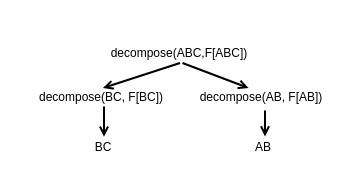
\includegraphics[scale=0.75]{decompose1.jpg}\\
 
Résultat:
\begin{itemize}
\item $R_{0}$ avec $schema(R_{0})=\{A,B\}$
\item $R_{1}$ avec $schema(R_{1})=\{B,C\}$
\end{itemize}


\subsection{Même questions pour $schema(R)=\{A,B,C,D\}$}
\subsubsection{Décomposition 3FN}
\begin{itemize}
\item $R_{0}$ avec $schema(R_{0})=\{A,B\}$
\item $R_{1}$ avec $schema(R_{1})=\{B,C\}$
\item $R_{2}$ avec $schema(R_{2})=\{A,B,C,D\}$
\end{itemize}
\subsubsection{Décomposition FNBC}
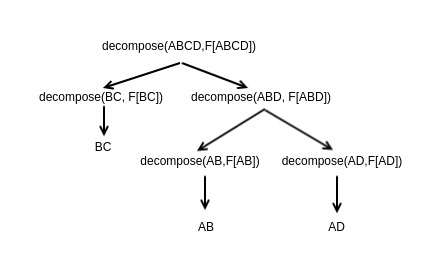
\includegraphics[scale=0.75]{decompose2.jpg}
Résultat:
\begin{itemize}
\item $R_{0}$ avec $schema(R_{0})=\{A,B\}$
\item $R_{1}$ avec $schema(R_{1})=\{B,C\}$
\item $R_{2}$ avec $schema(R_{2})=\{A,D\}$
\end{itemize}

\section{Relations d'Armstrong}
Soit $R$ un symbole de relation avec $schema(R)=\{A,B,C\}$. Soit $F$ un ensemble de F sur $R$ avec $F=\{A\rightarrow B, B\rightarrow C\}$.
\subsection{Donner une relation d'Armstrong $r_{0}$ pour $F$}
\begin{tabular}{c|c||c|c}
$A^{+}_{F}$ & $ABC$ & $AB^{+}_{F}$ & $ABC$ \\ 
$B^{+}_{F}$ & $BC$ & $AC^{+}_{F}$ & $ABC$ \\ 
$C^{+}_{F}$ & $C$ & $BC^{+}_{F}$ & $BC$ \\ 
\end{tabular} \\

Ainsi $CL(F)=\{\emptyset,C,BC,ABC\}$ donc $IRR(F)=\{\emptyset,C,BC\}$\\

\begin{tabular}{c|ccc}
$r_{0}$ & A & B & C \\ 
\hline 
$t_{0}$ & 0 & 0 & 0 \\ 
$t_{1}$ & 1 & 1 & 1 \\ 
$t_{2}$ & 2 & 2 & 0 \\ 
$t_{3}$ & 3 & 0 & 0 \\ 
\end{tabular} 

\subsubsection{De même pour $F=\{AB \rightarrow C, BC \rightarrow A\}$}
\begin{tabular}{c|c||c|c}
$A^{+}_{F}$ & $A$ & $AB^{+}_{F}$ & $ABC$ \\ 
$B^{+}_{F}$ & $BC$ & $AC^{+}_{F}$ & $AC$ \\ 
$C^{+}_{F}$ & $C$ & $BC^{+}_{F}$ & $ABC$ \\ 
\end{tabular} \\

Ainsi $CL(F)=\{\emptyset,A,B,C,AC,ABC\}$ donc $IRR(F)=\{A,B,C,AC\}$\\

\begin{tabular}{c|ccc}
$r_{0}$ & A & B & C \\ 
\hline 
$t_{0}$ & 0 & 0 & 0 \\ 
$t_{1}$ & 0 & 1 & 1 \\ 
$t_{2}$ & 2 & 0 & 2 \\ 
$t_{3}$ & 3 & 3 & 0 \\ 
$t_{4}$ & 0 & 4 & 0 \\ 
\end{tabular} 

\section{Conception à partir d'un texte}
Une conférence est organisée en différentes sessions, chaque session portant un nom et ayant en moyenne trois papiers. Un papier est caractérisé par un titre, une liste ordonnée d'auteurs et un nombre de pages et est présentée à une seule conférence. La session est dirigée par un président de session issu des membres du comité de programme. Chaque papier est évalué par plusieurs membres du comité de programme (CP). Une évaluation comporte une note et un commentaire.\\
Modéliser cette application en utilisant l'approche de conception dite de la relation universelle.

\subsection{Identifier les attributs décrivant l'univers du discours}
$U=\{conference, session, nomSession, papier, titrePapier, auteur, rangAuteur$\\
 $ nomAuteur, nPages, presSession, membreCP, nomMembre, evaluation, note, commentaire\}$

\subsection{Coder les contraintes avec des Dépendances Fonctionnelles}
Soit $F$ un ensemble de DF sur $U$,$F$ contient:
\begin{itemize}
\item $session \rightarrow conference$
\item $session \rightarrow nomSession$
\item $session \rightarrow presSession$
\item $papier \rightarrow titrePapier$
\item $papier \rightarrow nPages$
\item $papier \rightarrow session$
\item $papier,auteur \rightarrow rangAuteur$
\item $papier,rangAuteur \rightarrow auteur$
\item $auteur \rightarrow nomAuteur$
\item $membreCP \rightarrow nomMembre$
\item $membreCP,papier \rightarrow evaluation$
\item $evaluation \rightarrow note$
\item $evaluation \rightarrow commentaire$
\end{itemize}
La couverture minimale de $F$ est:
\begin{itemize}
\item $session \rightarrow conference,nomSession,presSession$
\item $papier \rightarrow titrePapier,nPages,session$
\item $papier,auteur \rightarrow rangAuteur$
\item $papier,rangAuteur \rightarrow auteur$
\item $auteur \rightarrow nomAuteur$
\item $membreCP \rightarrow nomMembre$
\item $membreCP,papier \rightarrow evaluation$
\item $evaluation \rightarrow note,commentaire$
\end{itemize}
\subsection{Proposer un schéma de base de données en 3FN}
Soit $R$ un symbole de base de données sur $U$,on trouve $schema(R)$ en 3FN avec l'algorithme de synthèse sur la couverture minimale de $F$ ci-dessus.\\
Résultat:
\begin{itemize}
\item $R_{0}$ avec $schema(R_{0})=\{session, conference, nomSession,presSession\}$
\item $R_{1}$ avec $schema(R_{1})=\{papier, titrePapier, nPages,session\}$
\item $R_{2}$ avec $schema(R_{2})=\{auteur, nomAuteur\}$
\item $R_{3}$ avec $schema(R_{1})=\{papier, auteur, rangAuteur\}$
\item $R_{4}$ avec $schema(R_{4})=\{membreCP, nomMembre\}$
\item $R_{5}$ avec $schema(R_{5})=\{membreCP, papier, evaluation\}$
\item $R_{6}$ avec $schema(R_{6})=\{evaluation,note,commentaire\}$
\end{itemize}

\end{document}